\documentclass{standalone}
\usepackage{tikz}
\usetikzlibrary{patterns, positioning}


\begin{document}
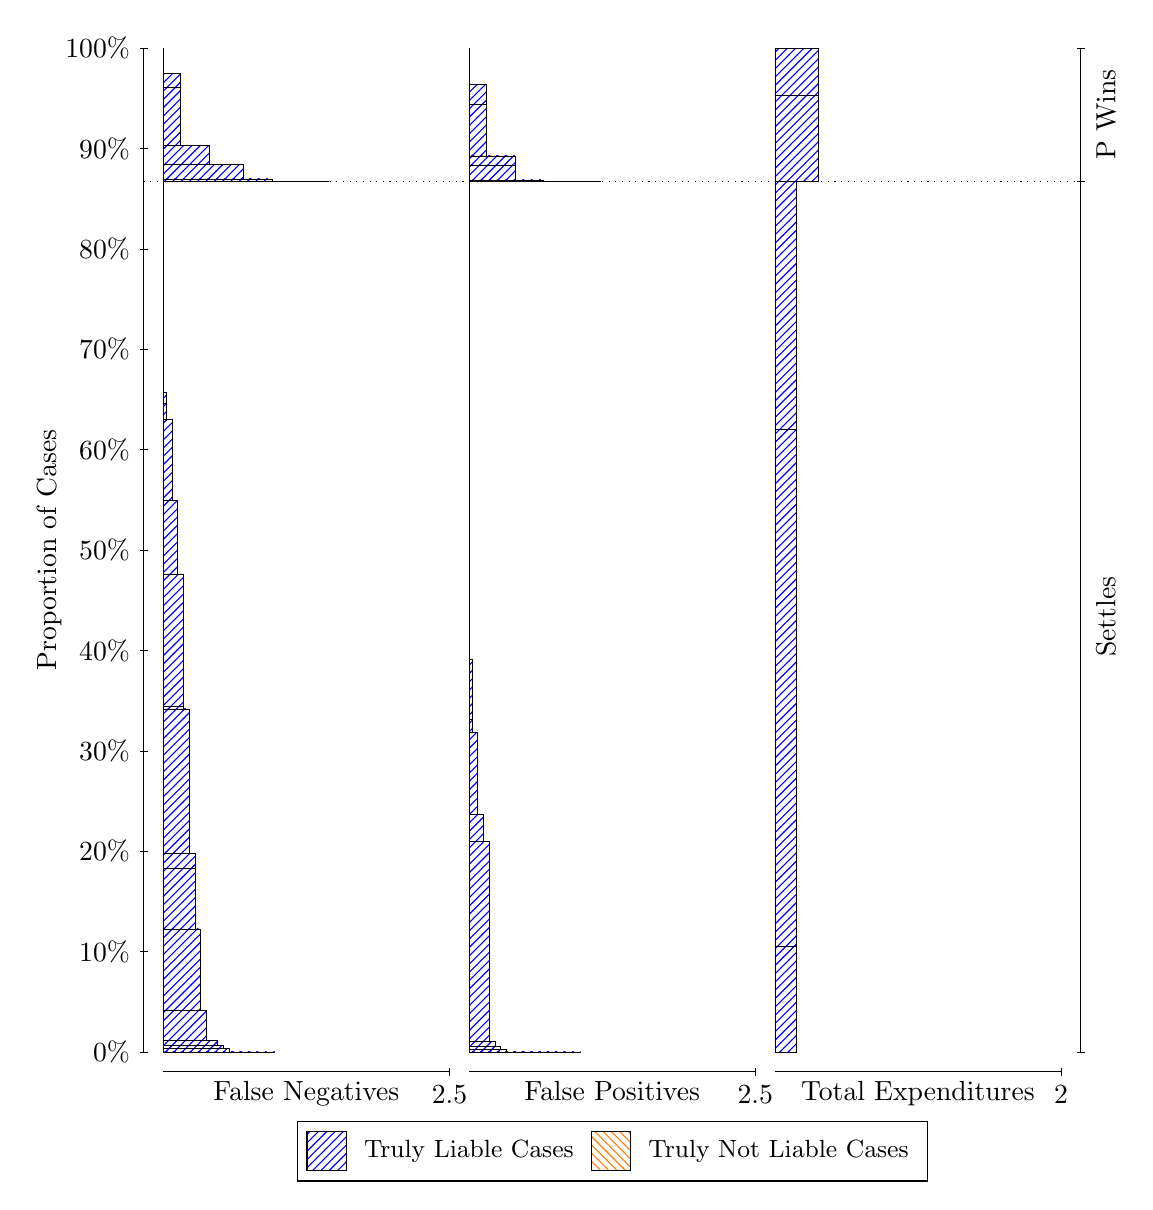
\begin{tikzpicture}
\draw[black, very thin] (1.5,1.75) -- (1.5,14.5);
\node[rotate=90, text=black, anchor=center] at (0.3, 8.125) {Proportion of Cases};
\draw[black, very thin] (1.45,1.75) -- (1.55,1.75);
\node[text=black, anchor=east] at (1.45, 1.75) {0\%};
\draw[black, very thin] (1.45,3.025) -- (1.55,3.025);
\node[text=black, anchor=east] at (1.45, 3.025) {10\%};
\draw[black, very thin] (1.45,4.3) -- (1.55,4.3);
\node[text=black, anchor=east] at (1.45, 4.3) {20\%};
\draw[black, very thin] (1.45,5.575) -- (1.55,5.575);
\node[text=black, anchor=east] at (1.45, 5.575) {30\%};
\draw[black, very thin] (1.45,6.85) -- (1.55,6.85);
\node[text=black, anchor=east] at (1.45, 6.85) {40\%};
\draw[black, very thin] (1.45,8.125) -- (1.55,8.125);
\node[text=black, anchor=east] at (1.45, 8.125) {50\%};
\draw[black, very thin] (1.45,9.4) -- (1.55,9.4);
\node[text=black, anchor=east] at (1.45, 9.4) {60\%};
\draw[black, very thin] (1.45,10.675) -- (1.55,10.675);
\node[text=black, anchor=east] at (1.45, 10.675) {70\%};
\draw[black, very thin] (1.45,11.95) -- (1.55,11.95);
\node[text=black, anchor=east] at (1.45, 11.95) {80\%};
\draw[black, very thin] (1.45,13.225) -- (1.55,13.225);
\node[text=black, anchor=east] at (1.45, 13.225) {90\%};
\draw[black, very thin] (1.45,14.5) -- (1.55,14.5);
\node[text=black, anchor=east] at (1.45, 14.5) {100\%};

\draw[black, very thin] (13.4,1.75) -- (13.4,14.5);
\draw[black, very thin] (13.35,1.75) -- (13.45,1.75);
\node[anchor=west] at (13.35, 1.75) {};
\draw[black, very thin] (13.35,12.806) -- (13.45,12.806);
\node[anchor=west] at (13.35, 12.806) {};
\draw[black, very thin] (13.35,14.5) -- (13.45,14.5);
\node[anchor=west] at (13.35, 14.5) {};

\draw[black, very thin, pattern color=blue, pattern=north east lines] (1.75,1.75) rectangle (3.167,1.75);
\draw[black, very thin, pattern color=blue, pattern=north east lines] (1.75,1.75) rectangle (3.0217,1.75);
\draw[black, very thin, pattern color=blue, pattern=north east lines] (1.75,1.75) rectangle (2.8763,1.75);
\draw[black, very thin, pattern color=blue, pattern=north east lines] (1.75,1.75) rectangle (2.8037,1.75);
\draw[black, very thin, pattern color=blue, pattern=north east lines] (1.75,1.75) rectangle (2.731,1.75);
\draw[black, very thin, pattern color=blue, pattern=north east lines] (1.75,1.75) rectangle (2.6583,1.7503);
\draw[black, very thin, pattern color=blue, pattern=north east lines] (1.75,1.7503) rectangle (2.5857,1.796);
\draw[black, very thin, pattern color=blue, pattern=north east lines] (1.75,1.796) rectangle (2.513,1.8291);
\draw[black, very thin, pattern color=blue, pattern=north east lines] (1.75,1.8291) rectangle (2.4403,1.8949);
\draw[black, very thin, pattern color=blue, pattern=north east lines] (1.75,1.8949) rectangle (2.3677,1.8961);
\draw[black, very thin, pattern color=blue, pattern=north east lines] (1.75,1.8961) rectangle (2.295,2.2739);
\draw[black, very thin, pattern color=blue, pattern=north east lines] (1.75,2.2739) rectangle (2.2223,3.3138);
\draw[black, very thin, pattern color=blue, pattern=north east lines] (1.75,3.3138) rectangle (2.1497,4.0779);
\draw[black, very thin, pattern color=blue, pattern=north east lines] (1.75,4.0779) rectangle (2.1497,4.2714);
\draw[black, very thin, pattern color=blue, pattern=north east lines] (1.75,4.2714) rectangle (2.077,6.1072);
\draw[black, very thin, pattern color=blue, pattern=north east lines] (1.75,6.1072) rectangle (2.0043,6.139);
\draw[black, very thin, pattern color=blue, pattern=north east lines] (1.75,6.139) rectangle (2.0043,7.8179);
\draw[black, very thin, pattern color=blue, pattern=north east lines] (1.75,7.8179) rectangle (1.9317,8.7516);
\draw[black, very thin, pattern color=blue, pattern=north east lines] (1.75,8.7516) rectangle (1.859,9.7887);
\draw[black, very thin, pattern color=blue, pattern=north east lines] (1.75,9.7887) rectangle (1.7863,9.9907);
\draw[black, very thin, pattern color=blue, pattern=north east lines] (1.75,9.9907) rectangle (1.7863,10.128);
\draw[black, very thin, pattern color=orange, pattern=north west lines] (1.75,10.128) rectangle (1.75,10.128);
\draw[black, very thin, pattern color=blue, pattern=north east lines] (1.75,10.128) rectangle (1.75,12.806);
\draw[black, very thin, pattern color=blue, pattern=north east lines] (1.75,12.806) rectangle (3.8573,12.806);
\draw[black, very thin, pattern color=blue, pattern=north east lines] (1.75,12.806) rectangle (3.494,12.806);
\draw[black, very thin, pattern color=blue, pattern=north east lines] (1.75,12.806) rectangle (3.1307,12.839);
\draw[black, very thin, pattern color=blue, pattern=north east lines] (1.75,12.839) rectangle (3.058,12.839);
\draw[black, very thin, pattern color=blue, pattern=north east lines] (1.75,12.839) rectangle (2.7673,13.023);
\draw[black, very thin, pattern color=blue, pattern=north east lines] (1.75,13.023) rectangle (2.6947,13.024);
\draw[black, very thin, pattern color=blue, pattern=north east lines] (1.75,13.024) rectangle (2.404,13.027);
\draw[black, very thin, pattern color=blue, pattern=north east lines] (1.75,13.027) rectangle (2.3313,13.266);
\draw[black, very thin, pattern color=blue, pattern=north east lines] (1.75,13.266) rectangle (2.0407,13.266);
\draw[black, very thin, pattern color=blue, pattern=north east lines] (1.75,13.266) rectangle (1.968,14.004);
\draw[black, very thin, pattern color=blue, pattern=north east lines] (1.75,14.004) rectangle (1.968,14.177);
\draw[black, very thin, pattern color=orange, pattern=north west lines] (1.75,14.177) rectangle (1.75,14.177);
\draw[black, very thin, pattern color=blue, pattern=north east lines] (1.75,14.177) rectangle (1.75,14.5);
\draw[black, very thin, pattern color=orange, pattern=north west lines] (5.6333,1.75) rectangle (7.0503,1.75);
\draw[black, very thin, pattern color=blue, pattern=north east lines] (5.6333,1.75) rectangle (7.0503,1.75);
\draw[black, very thin, pattern color=orange, pattern=north west lines] (5.6333,1.75) rectangle (6.905,1.75);
\draw[black, very thin, pattern color=blue, pattern=north east lines] (5.6333,1.75) rectangle (6.905,1.75);
\draw[black, very thin, pattern color=orange, pattern=north west lines] (5.6333,1.75) rectangle (6.7597,1.75);
\draw[black, very thin, pattern color=blue, pattern=north east lines] (5.6333,1.75) rectangle (6.7597,1.75);
\draw[black, very thin, pattern color=blue, pattern=north east lines] (5.6333,1.75) rectangle (6.687,1.75);
\draw[black, very thin, pattern color=orange, pattern=north west lines] (5.6333,1.75) rectangle (6.6143,1.75);
\draw[black, very thin, pattern color=blue, pattern=north east lines] (5.6333,1.75) rectangle (6.6143,1.75);
\draw[black, very thin, pattern color=blue, pattern=north east lines] (5.6333,1.75) rectangle (6.5417,1.75);
\draw[black, very thin, pattern color=orange, pattern=north west lines] (5.6333,1.75) rectangle (6.469,1.75);
\draw[black, very thin, pattern color=blue, pattern=north east lines] (5.6333,1.75) rectangle (6.469,1.75);
\draw[black, very thin, pattern color=blue, pattern=north east lines] (5.6333,1.75) rectangle (6.3963,1.75);
\draw[black, very thin, pattern color=orange, pattern=north west lines] (5.6333,1.75) rectangle (6.3237,1.75);
\draw[black, very thin, pattern color=blue, pattern=north east lines] (5.6333,1.75) rectangle (6.3237,1.75);
\draw[black, very thin, pattern color=blue, pattern=north east lines] (5.6333,1.75) rectangle (6.251,1.75);
\draw[black, very thin, pattern color=orange, pattern=north west lines] (5.6333,1.75) rectangle (6.1783,1.75);
\draw[black, very thin, pattern color=blue, pattern=north east lines] (5.6333,1.75) rectangle (6.1783,1.7523);
\draw[black, very thin, pattern color=blue, pattern=north east lines] (5.6333,1.7523) rectangle (6.1057,1.7848);
\draw[black, very thin, pattern color=orange, pattern=north west lines] (5.6333,1.7848) rectangle (6.033,1.7848);
\draw[black, very thin, pattern color=blue, pattern=north east lines] (5.6333,1.7848) rectangle (6.033,1.7868);
\draw[black, very thin, pattern color=blue, pattern=north east lines] (5.6333,1.7868) rectangle (6.033,1.8198);
\draw[black, very thin, pattern color=blue, pattern=north east lines] (5.6333,1.8198) rectangle (5.9603,1.8845);
\draw[black, very thin, pattern color=orange, pattern=north west lines] (5.6333,1.8845) rectangle (5.8877,1.8845);
\draw[black, very thin, pattern color=blue, pattern=north east lines] (5.6333,1.8845) rectangle (5.8877,4.4264);
\draw[black, very thin, pattern color=blue, pattern=north east lines] (5.6333,4.4264) rectangle (5.8877,4.4275);
\draw[black, very thin, pattern color=blue, pattern=north east lines] (5.6333,4.4275) rectangle (5.815,4.7668);
\draw[black, very thin, pattern color=blue, pattern=north east lines] (5.6333,4.7668) rectangle (5.7423,5.804);
\draw[black, very thin, pattern color=blue, pattern=north east lines] (5.6333,5.804) rectangle (5.6697,5.9729);
\draw[black, very thin, pattern color=blue, pattern=north east lines] (5.6333,5.9729) rectangle (5.6697,6.7377);
\draw[black, very thin, pattern color=blue, pattern=north east lines] (5.6333,6.7377) rectangle (5.6333,12.806);
\draw[black, very thin, pattern color=orange, pattern=north west lines] (5.6333,12.806) rectangle (7.3047,12.806);
\draw[black, very thin, pattern color=blue, pattern=north east lines] (5.6333,12.806) rectangle (7.3047,12.806);
\draw[black, very thin, pattern color=orange, pattern=north west lines] (5.6333,12.806) rectangle (6.9413,12.806);
\draw[black, very thin, pattern color=blue, pattern=north east lines] (5.6333,12.806) rectangle (6.9413,12.806);
\draw[black, very thin, pattern color=blue, pattern=north east lines] (5.6333,12.806) rectangle (6.9413,12.806);
\draw[black, very thin, pattern color=orange, pattern=north west lines] (5.6333,12.806) rectangle (6.578,12.806);
\draw[black, very thin, pattern color=blue, pattern=north east lines] (5.6333,12.806) rectangle (6.578,12.814);
\draw[black, very thin, pattern color=blue, pattern=north east lines] (5.6333,12.814) rectangle (6.578,12.824);
\draw[black, very thin, pattern color=orange, pattern=north west lines] (5.6333,12.824) rectangle (6.2147,12.824);
\draw[black, very thin, pattern color=blue, pattern=north east lines] (5.6333,12.824) rectangle (6.2147,13.016);
\draw[black, very thin, pattern color=blue, pattern=north east lines] (5.6333,13.016) rectangle (6.2147,13.129);
\draw[black, very thin, pattern color=orange, pattern=north west lines] (5.6333,13.129) rectangle (6.142,13.129);
\draw[black, very thin, pattern color=blue, pattern=north east lines] (5.6333,13.129) rectangle (6.142,13.129);
\draw[black, very thin, pattern color=blue, pattern=north east lines] (5.6333,13.129) rectangle (5.8513,13.781);
\draw[black, very thin, pattern color=blue, pattern=north east lines] (5.6333,13.781) rectangle (5.8513,14.039);
\draw[black, very thin, pattern color=orange, pattern=north west lines] (5.6333,14.039) rectangle (5.7787,14.039);
\draw[black, very thin, pattern color=blue, pattern=north east lines] (5.6333,14.039) rectangle (5.7787,14.039);
\draw[black, very thin, pattern color=blue, pattern=north east lines] (5.6333,14.039) rectangle (5.7787,14.039);
\draw[black, very thin, pattern color=orange, pattern=north west lines] (5.6333,14.039) rectangle (5.6333,14.039);
\draw[black, very thin, pattern color=blue, pattern=north east lines] (5.6333,14.039) rectangle (5.6333,14.5);
\draw[black, very thin, pattern color=orange, pattern=north west lines] (9.5167,1.75) rectangle (9.7892,1.75);
\draw[black, very thin, pattern color=blue, pattern=north east lines] (9.5167,1.75) rectangle (9.7892,3.0951);
\draw[black, very thin, pattern color=orange, pattern=north west lines] (9.5167,3.0951) rectangle (9.7892,3.0951);
\draw[black, very thin, pattern color=blue, pattern=north east lines] (9.5167,3.0951) rectangle (9.7892,9.6605);
\draw[black, very thin, pattern color=orange, pattern=north west lines] (9.5167,9.6605) rectangle (9.7892,9.6605);
\draw[black, very thin, pattern color=blue, pattern=north east lines] (9.5167,9.6605) rectangle (9.7892,12.806);
\draw[black, very thin, pattern color=orange, pattern=north west lines] (9.5167,12.806) rectangle (10.062,12.806);
\draw[black, very thin, pattern color=blue, pattern=north east lines] (9.5167,12.806) rectangle (10.062,13.896);
\draw[black, very thin, pattern color=orange, pattern=north west lines] (9.5167,13.896) rectangle (10.062,13.896);
\draw[black, very thin, pattern color=blue, pattern=north east lines] (9.5167,13.896) rectangle (10.062,14.5);
\draw[black, dotted] (1.5,12.806) -- (13.4,12.806);
\draw[black, very thin] (1.75,1.5) -- (5.3833,1.5);
\node[text=black, anchor=north] at (3.5667, 1.5) {False Negatives};
\draw[black, very thin] (5.3833,1.45) -- (5.3833,1.55);
\node[text=black, anchor=north] at (5.3833, 1.45) {2.5};

\draw[black, very thin] (5.6333,1.5) -- (9.2667,1.5);
\node[text=black, anchor=north] at (7.45, 1.5) {False Positives};
\draw[black, very thin] (9.2667,1.45) -- (9.2667,1.55);
\node[text=black, anchor=north] at (9.2667, 1.45) {2.5};

\draw[black, very thin] (9.5167,1.5) -- (13.15,1.5);
\node[text=black, anchor=north] at (11.333, 1.5) {Total Expenditures};
\draw[black, very thin] (13.15,1.45) -- (13.15,1.55);
\node[text=black, anchor=north] at (13.15, 1.45) {2};

\node[text=black, centered, rotate=90] at (13.72, 7.2778) {Settles};
\node[text=black, centered, rotate=90] at (13.72, 13.653) {P Wins};

\draw (7.449999999999999,1.5) node[draw=none] (baseCoordinate) {};
\begin{scope}[align=center]
        \matrix[scale=0.5, draw=black, below=0.5cm of baseCoordinate, nodes={draw}, column sep=0.1cm]{
            \node[rectangle, draw, minimum width=0.5cm, minimum height=0.5cm, pattern color=blue, pattern=north east lines] {}; &
            \node[draw=none, font=\small, text=black] (B) {Truly Liable Cases}; &
            \node[rectangle, draw, minimum width=0.5cm, minimum height=0.5cm, pattern color=orange, pattern=north west lines] {}; &
            \node[draw=none, font=\small, text=black] (B) {Truly Not Liable Cases}; \\
            };
\end{scope}

\end{tikzpicture}
\end{document}